\documentclass[12pt, letterpaper, oneside]{article}
\usepackage[affil-it]{authblk}
\usepackage{graphicx}
\usepackage{xeCJK}

\setCJKmainfont{ukai.ttc}
\setCJKmonofont{ukai.ttc}

\title{Final Report on Algorithmic Trading}
\author{Tran Phong Binh\thanks{Email: \texttt{phongbinh2511@gmail.com}}}
\affil{Department of Computer Science and Information Technology,
National Taipei University of Technology, Taipei}
\date{\today}

\begin{document}

\maketitle

\begin{abstract}
We briefly explain and analyze the paper \textit{Using Reinforcement Learning in the Algorithmic Trading Problem}\cite{a3c_trading}, which applied the asynchronous advantage actor-critic (A3C) method into trading and claimed to have attained a strategy of 66\% profitability per annum. We then investigate five trading strategies that were developed throughout the course with empirical experimental results.
\end{abstract}

\section{Introduction}
My work begins with a brief description for the research \textit{Using Reinforcement Learning in the Algorithmic Trading Problem}, along with a few personal analyses on the composition of the paper. In addition, five trading strategies assigned by the lecturer of the course will also be provided, with their performances being visually compared. The report concludes with some thoughts of my own on the progress of researching and working on the said article and the five strategies.

\section{Paper}
This section focuses on presenting and analyzing the paper \textit{Using Reinforcement Learning in the Algorithmic Trading Problem}.

\subsection{Description}
\textit{Using Reinforcement Learning in the Algorithmic Trading Problem} is an experimental work applying long short-term memory (LSTM) and reinforcement learning (RL) with A3C into trading. The paper is written by three Russian researchers from the Skolkovo Institute of Science and Technology, Moscow (with one also holding a position at the Marchuk Institute of Numerical Mathematics, Russian Academy of Sciences, Moscow). The paper is published on 26th June 2019 in the \textit{Journal of Communications Technology and Electronics} (by Pleiades Publishing, Inc.). The motivation and contribution of the paper is identical -- while LSTM and RL with various reinforced learning algorithms, such as Q-learning\cite{q_learning}, Deep Q-learning\cite{deep}, and other actor-critic methods\cite{ac1, ac2} have been applied into trading, the application of A3C into trading has yet been seen in the literature; thus, this paper contributes by carrying on the task.

This paper is purely experimental; that is, it has no comparisons of performances between the aforementioned algorithms applied into trading, nor it has any theoretical analyses on the usage of A3C in trading. The authors use LSTM and RL with A3C to train models for a designated trading problem, which is defined as follows:
\begin{itemize}
    \item The model trades on futures of MOEX:RTSI\footnote{MOEX stands for Moscow Exchange, while RTSI stands for Russian Trading System Index} from 15th December 2015 to 15th June 2016.
    \item The model makes a trading decision every minute (3 trading decisions are available: long -- do nothing, neutral -- sell out all holding futures, and short -- buy in a fixed volume of futures).
    \item The model accounts for a fixed commission fee of 2.50 Russian rubles per transaction (which I assume to begin with a short and end with a neutral).
\end{itemize}
The trained models are supposed to maximize profitability. The paper's sole goal is straightforward: to experiment various neural network architectures of LSTM and RL with A3C to find the model yielding the highest profitability. The authors claim the best model yielding a profitability of 66\% per annum, which is shown in Table \ref{table:data} below:

\begin{table}[h!]
    \centering
    \begin{tabular}{ |c|c| }
        \hline
        Neural network architecture & Profit per annum (\%) \\ [0.5ex]
        \hline
        5 & 5.2 \\
        8 & 28.4 \\
        5coolV & 20.7 \\
        9 & \textbf{66.5} \\
        6 & -143.7 \\ [0.5ex]
        \hline
    \end{tabular}
    \caption{Result of execution on six-month test data}
    \label{table:data}
\end{table}

\subsection{Analyses}
There are, however, many flaws in this paper. Some of them are:
\begin{enumerate}
    \item The maths in the paper seriously lack clarification, with mathematical notations being used inconsistently throughout section 2.
    \item The dropout method is misused -- it is not for getting better optimization objectives, but for getting to an optimization objective faster.
    \item The date ranges of the financial instrument used for training and testing models are suspiciously hyperparameters.
    \item The mechanism for initializing the weights of the neural networks is not provided.
    \item A concrete definition for transaction and commission fee is not given.
    \item All figures lack sufficient clarification.
\end{enumerate}
The journal which accepted the article -- \textit{Journal of Communications Technology and Electronics} -- is also of poor condition, with its impact factor in 2019 being 0.483\cite{comtech}. Given these, we can conclude that this is not a quality and robust research.

\section{Strategies}
This section describes and compares the performances of the five trading strategies, consisting of two countertrend and three trend trading systems. All strategies are designed to trade on a daily basis for the top 12 stocks of Taiwan exchange-traded fund (ETF) 0050, which is listed in Table \ref{table:stock}. The stock data is collected from the laboratory iLoveTradingLab, Department of Information and Finance Management, National Taipei University of Technology, ranging from each stock's date of initial public offering (IPO) to 11th September 2020. The profit/loss vectors are depicted, with several other metrices calculated, including the win rate, gain rate, profit factor, mean drawdown (MDD), and the maximum drawdown duration (Max DDD). The source code is also available on GitHub\footnote{\texttt{https://github.com/phogbinh/NTUT2020FallAlgorithmicTrading}} under the \texttt{ifm} directory.

\begin{table}[h!]
    \centering
    \begin{tabular}{ |c|p{10ex}|p{40ex}|c| }
        \hline
        No. & Company & Company (in English) & Symbol \\ [0.5ex]
        \hline
        1 & 台積電 & TSMC Limited & 2330 \\
        2 & 聯發科 & MediaTek Inc. & 2454 \\
        3 & 鴻海 & Hon Hai Precision Industry Co., Ltd. & 2317 \\
        4 & 台達電 & Delta Electronics, Inc. & 2308 \\
        5 & 聯電 & United Microelectronics Corporation & 2303 \\
        6 & 台塑 & Formosa Plastics Corporation & 1301 \\
        7 & 中華電 & Chunghwa Telecom Co., Ltd. & 2412 \\
        8 & 南亞 & Nan Ya Plastics Corporation & 1303 \\
        9 & 中信金 & CTBC Financial Holding Co., Ltd. & 2891 \\
        10 & 國泰金 & Cathay Financial Holding Co., Ltd. & 2882 \\
        11 & 大立光 & LARGAN Precision Co.,Ltd & 3008 \\
        12 & 富邦金 & Fubon Financial Holding Co., Ltd. & 2881 \\ [0.5ex]
        \hline
    \end{tabular}
    \caption{Top 12 stocks of Taiwan ETF 0050}
    \label{table:stock}
\end{table}

\subsection{Strategy A -- Countertrend trading}
When the closing price of the given stock is strictly less than the lowest low of the previous 5 days (not including today), if we haven't bought any shares of the stock, we buy in 1,000 shares (1 trading unit in Taiwan, later referred as 1 ticket) at opening price on the next day. Later each time this happens, we take an amount equivalent to all the money having used to acquire the tickets of the stock, and buy in as much as we can at opening price on the next day. When the closing price of the given stock is strictly greater than the highest high of the previous 3 days (not including today), we sell out all of our tickets at opening price on the following day (note that we consider this as resetting the money having used to acquire the tickets of the stock to 0). The performance of strategy A is demonstrated in Figure \ref{fig:a} and Table \ref{table:a}.

\begin{figure}[h]
    \centering
    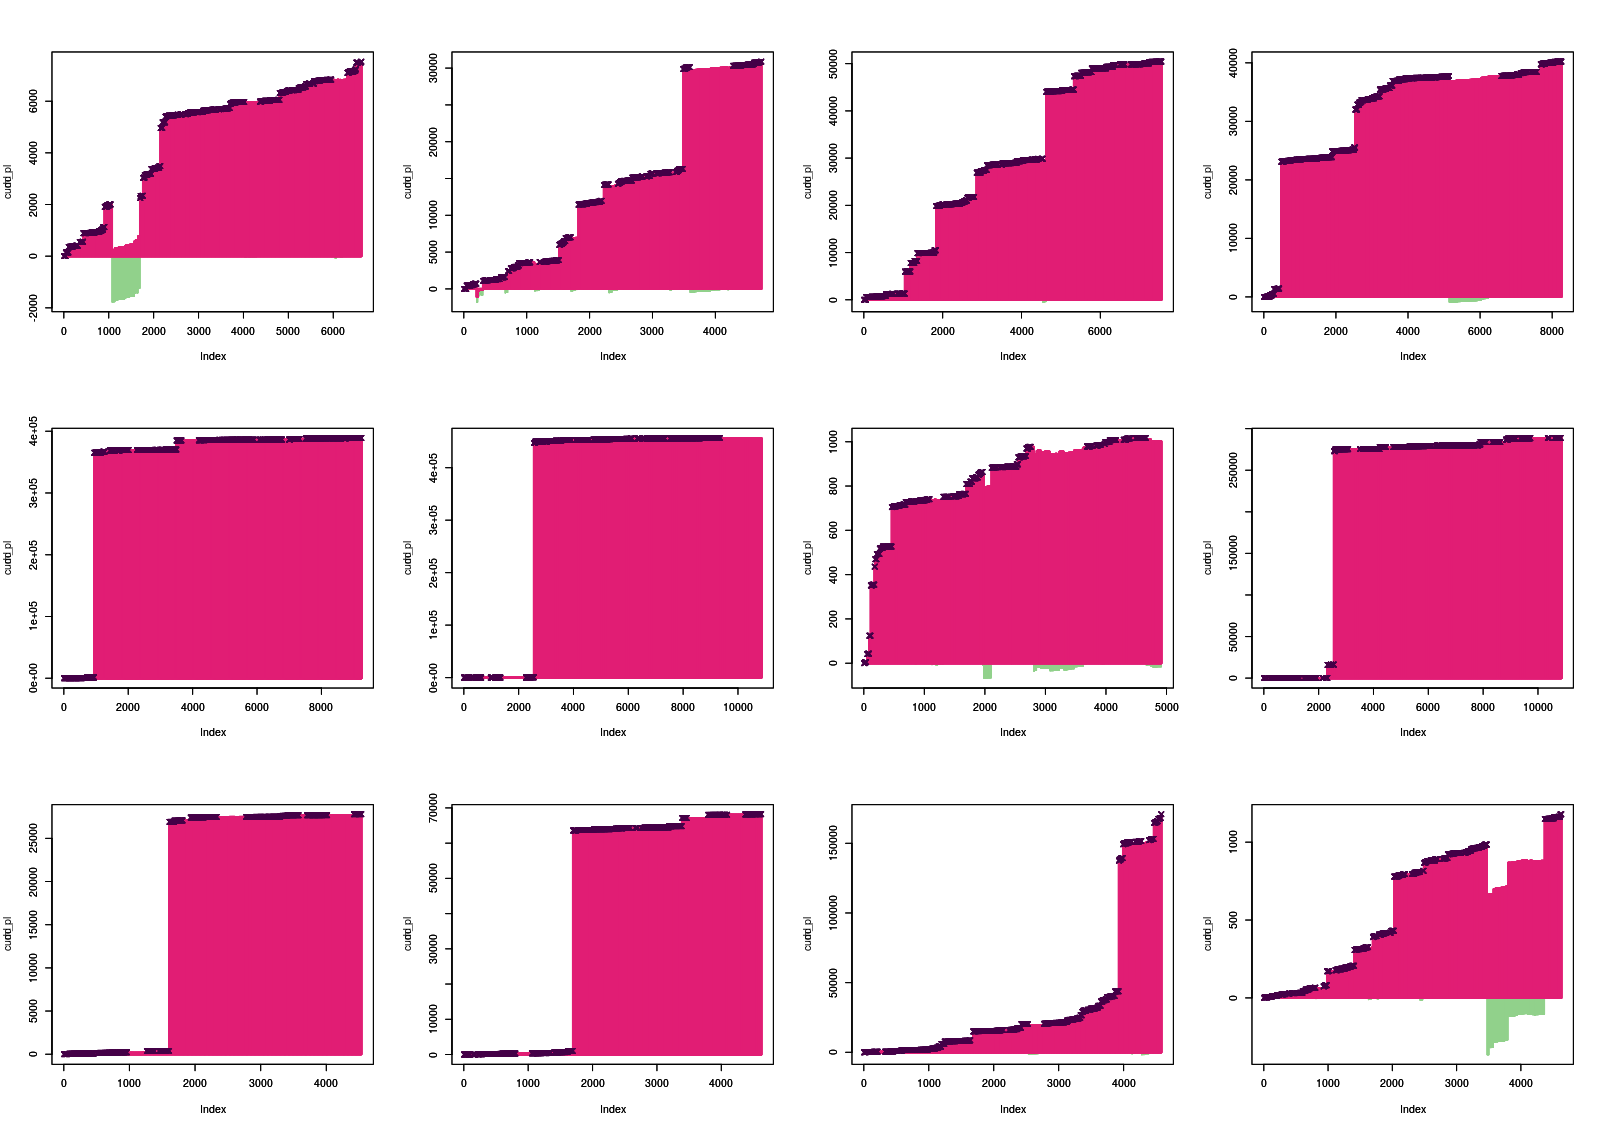
\includegraphics[width=0.75\textwidth]{sa_pl}
    \caption{Profit/loss vector of strategy A}
    \label{fig:a}
\end{figure}

\begin{table}[h!]
    \centering
    \begin{tabular}{ |c|c|c|c|c|c| }
        \hline
        Symbol & Win rate & Gain rate & Profit factor & MDD & Max DDD \\ [0.5ex]
        \hline
        2330 & 0.88 & 0.62 & 4.68 & -150.89 & 652 \\
        2454 & 0.89 & 0.89 & 7.78 & -78.59 & 683 \\
        2317 & 0.92 & 5.61 & 69.05 & -6.21 & 157 \\
        2308 & 0.94 & 2.27 & 36.96 & -90.77 & 1446 \\
        2303 & 0.89 & 47.22 & 414.63 & -20.02 & 534 \\
        1301 & 0.85 & 39.07 & 226.40 & -187.76 & 925 \\
        2412 & 0.76 & 1.95 & 6.53 & -6.82 & 925 \\
        1303 & 0.87 & 49.49 & 349.30 & -9.97 & 632 \\
        2891 & 0.86 & 41.94 & 257.88 & -4.73 & 441 \\
        2882 & 0.85 & 78.49 & 465.75 & -4.88 & 327 \\
        3008 & 0.92 & 3.10 & 38.84 & -100.58 & 240 \\
        2881 & 0.86 & 0.56 & 3.75 & -34.49 & 897 \\ [0.5ex]
        \hline
    \end{tabular}
    \caption{Performance metrices of strategy A, with MDD's unit being New Taiwan Dollar (NTD) and Max DDD's unit being day}
    \label{table:a}
\end{table}

\subsection{Strategy B -- Countertrend trading}
Long-term moving average is 17-day zero lag exponential moving average (ZLEMA) of closing price of the given stock, while short-term moving average is 9-day. When short-term moving average crosses below long-term moving average (death cross), we buy in at opening price on the next day, and then hold to sell out at opening price on the following day when short-term moving average crosses above long-term moving average (golden cross). The performance of strategy B is demonstrated in Figure \ref{fig:b} and Table \ref{table:b}.

\begin{figure}[h]
    \centering
    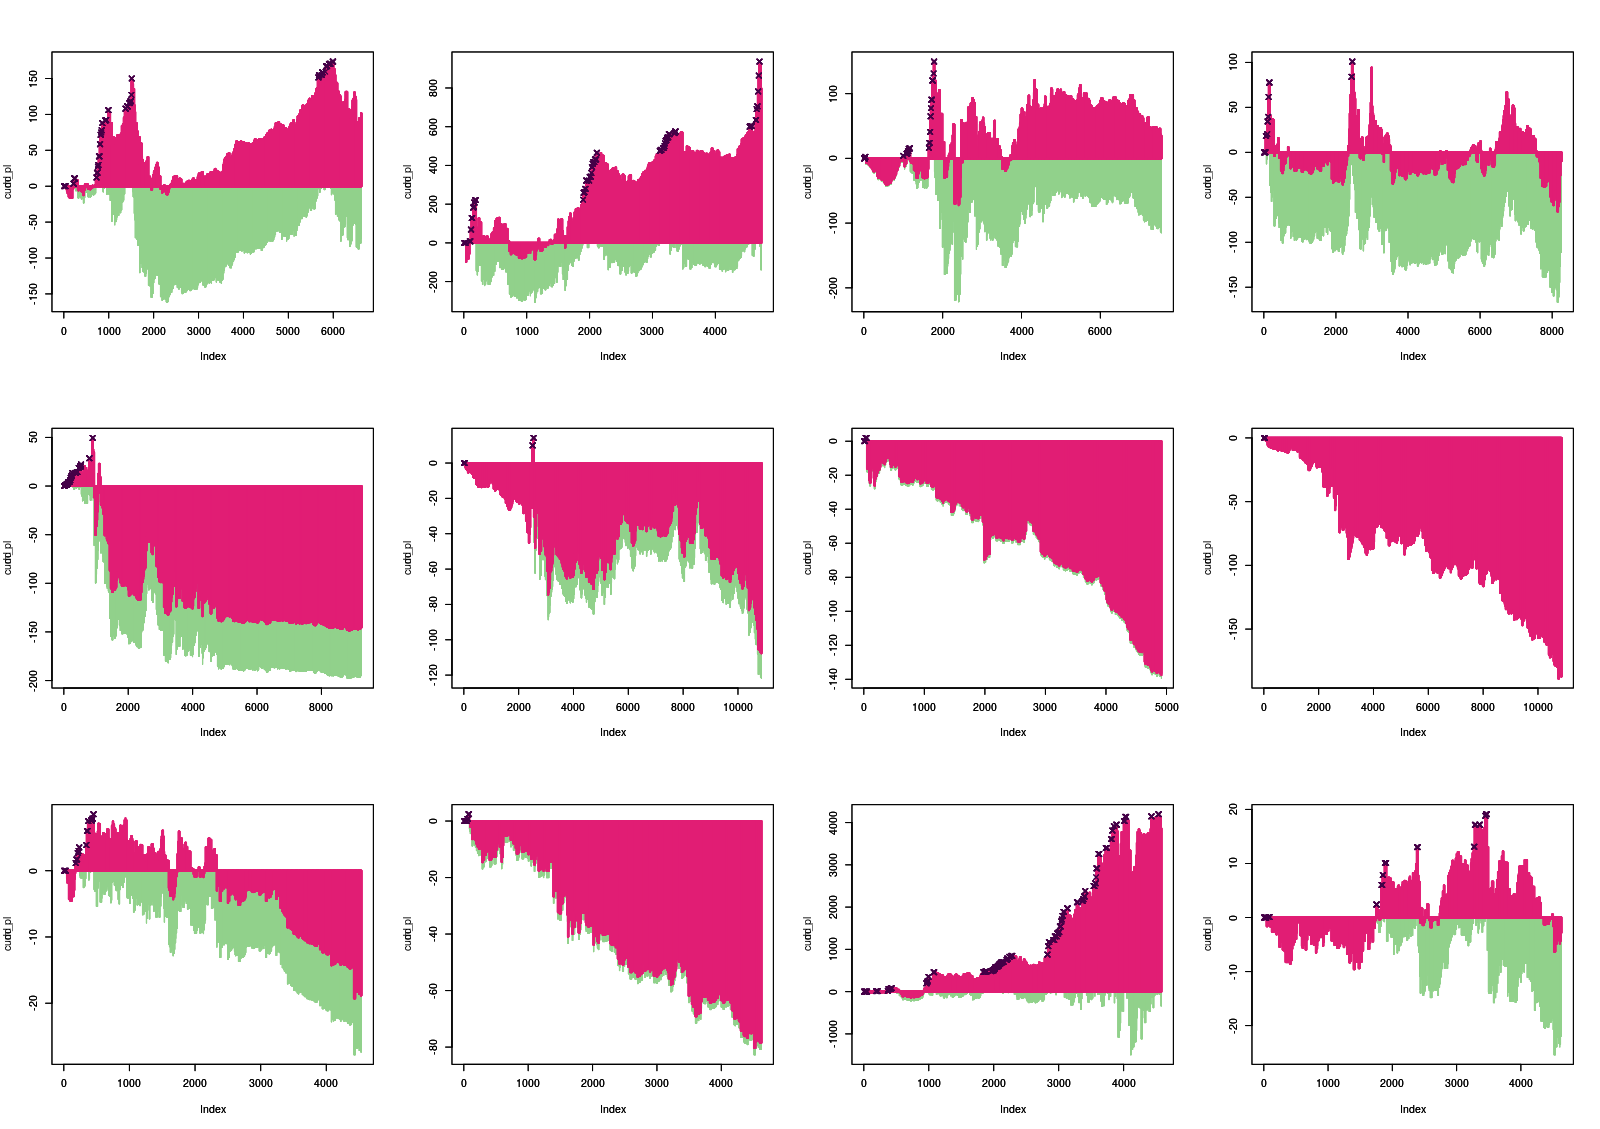
\includegraphics[width=0.75\textwidth]{sb_pl}
    \caption{Profit/loss vector of strategy B}
    \label{fig:b}
\end{figure}

\begin{table}[h!]
    \centering
    \begin{tabular}{ |c|c|c|c|c|c| }
        \hline
        Symbol & Win rate & Gain rate & Profit factor & MDD & Max DDD \\ [0.5ex]
        \hline
        2330 & 0.64 & 0.61 & 1.12 & -71.33 & 4149 \\
        2454 & 0.63 & 0.74 & 1.31 & -113.32 & 1699 \\
        2317 & 0.57 & 0.74 & 1.02 & -73.57 & 948 \\
        2308 & 0.56 & 0.74 & 0.99 & -96.54 & 2265 \\
        2303 & 0.54 & 0.69 & 0.83 & -151.81 & 244 \\
        1301 & 0.51 & 0.81 & 0.86 & -51.96 & 2465 \\
        2412 & 0.43 & 0.70 & 0.53 & -61.34 & 1 \\
        1303 & 0.52 & 0.68 & 0.75 & -83.51 & 1 \\
        2891 & 0.51 & 0.77 & 0.83 & -10.52 & 143 \\
        2882 & 0.53 & 0.61 & 0.71 & -41.97 & 1 \\
        3008 & 0.61 & 0.87 & 1.41 & -143.73 & 750 \\
        2881 & 0.57 & 0.72 & 0.98 & -7.20 & 1653 \\ [0.5ex]
        \hline
    \end{tabular}
    \caption{Performance metrices of strategy B, with MDD's unit being NTD and Max DDD's unit being day}
    \label{table:b}
\end{table}

\subsection{Strategy C -- Trend trading}
Long-term moving average is 56-day simple moving average (SMA) of closing price of the given stock, while short-term moving average is 42-day exponential moving average (EMA). When short-term moving average crosses above long-term moving average (golden cross), we buy in at opening price on the next day, and then hold to sell out at opening price on the following day when short-term moving average crosses below long-term moving average (death cross). The performance of strategy C is demonstrated in Figure \ref{fig:c} and Table \ref{table:c}.

\begin{figure}[h]
    \centering
    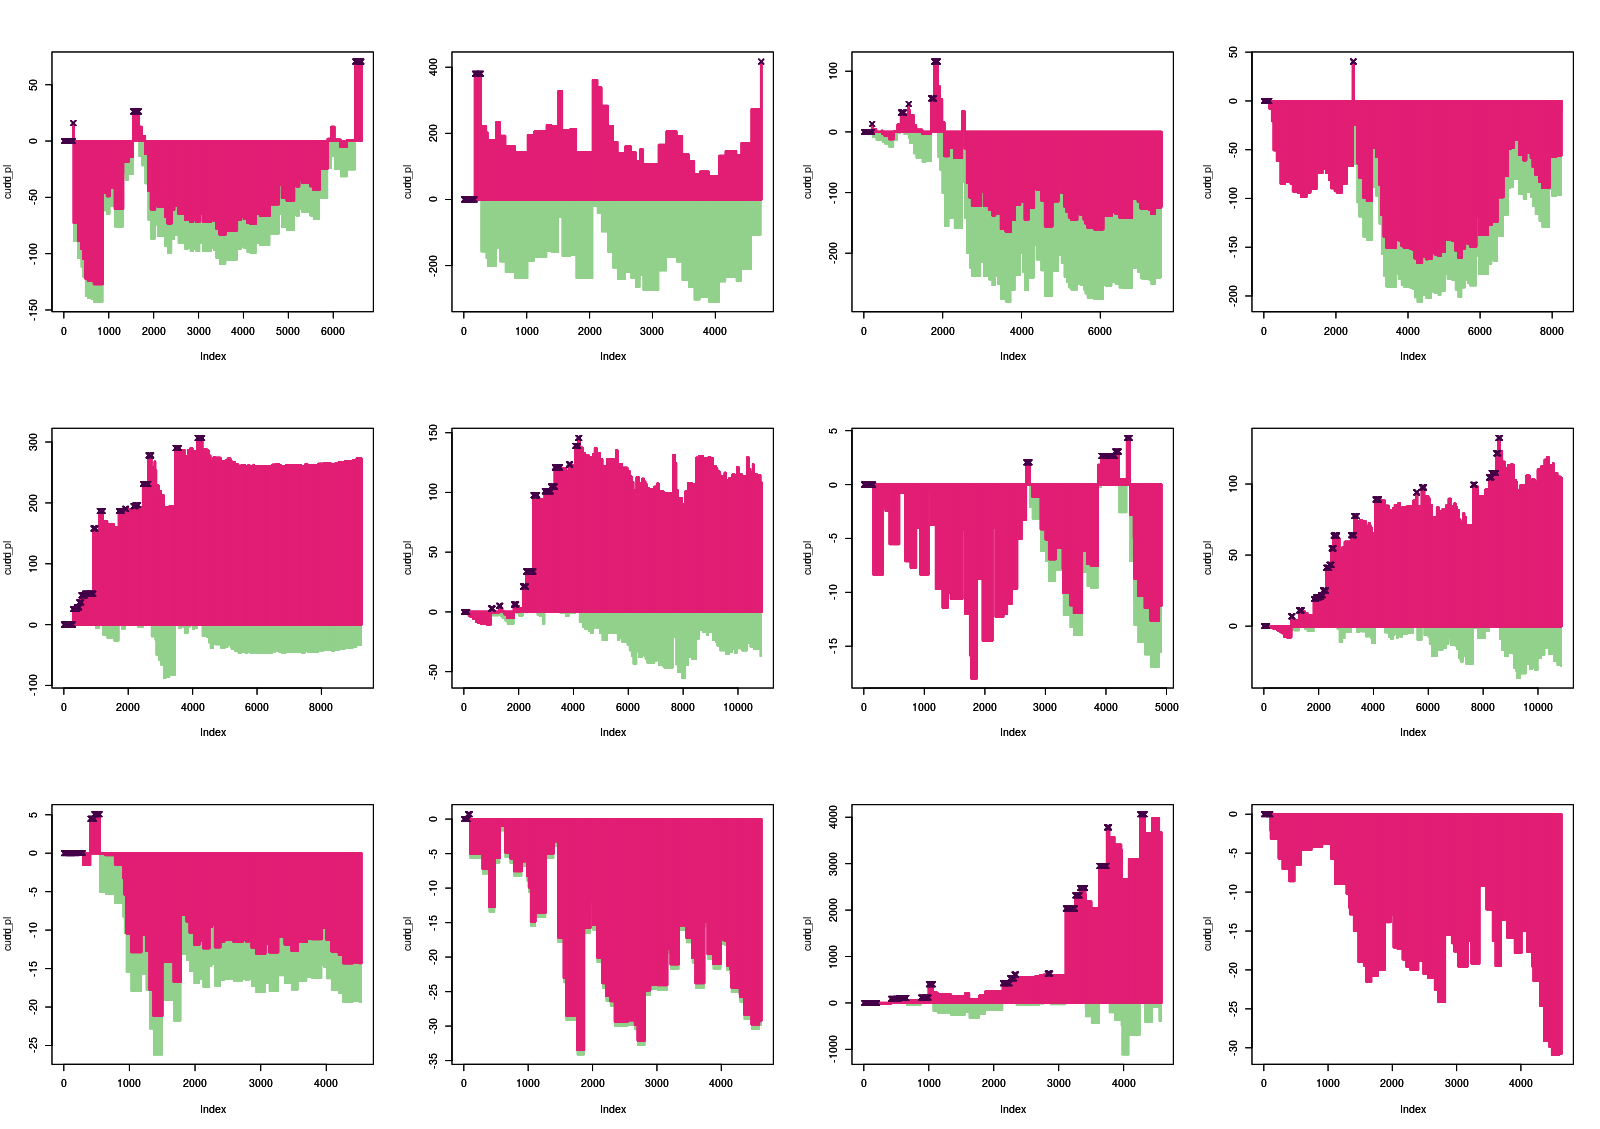
\includegraphics[width=0.75\textwidth]{sc_pl}
    \caption{Profit/loss vector of strategy C}
    \label{fig:c}
\end{figure}

\begin{table}[h!]
    \centering
    \begin{tabular}{ |c|c|c|c|c|c| }
        \hline
        Symbol & Win rate & Gain rate & Profit factor & MDD & Max DDD \\ [0.5ex]
        \hline
        2330 & 0.38 & 1.87 & 1.19 & -73.14 & 4813 \\
        2454 & 0.44 & 1.81 & 1.43 & -194.93 & 4450 \\
        2317 & 0.32 & 1.77 & 0.84 & -177.60 & 723 \\
        2308 & 0.35 & 1.74 & 0.98 & -128.24 & 2313 \\
        2303 & 0.48 & 2.31 & 2.16 & -29.16 & 749 \\
        1301 & 0.34 & 2.69 & 1.44 & -19.52 & 863 \\
        2412 & 0.37 & 1.47 & 0.88 & -7.95 & 2524 \\
        1303 & 0.44 & 1.97 & 1.55 & -10.02 & 1784 \\
        2891 & 0.37 & 1.21 & 0.72 & -14.48 & 110 \\
        2882 & 0.31 & 1.59 & 0.73 & -19.10 & 1 \\
        3008 & 0.52 & 2.10 & 2.29 & -158.73 & 1073 \\
        2881 & 0.29 & 1.53 & 0.63 & -14.96 & 1 \\ [0.5ex]
        \hline
    \end{tabular}
    \caption{Performance metrices of strategy C, with MDD's unit being NTD and Max DDD's unit being day}
    \label{table:c}
\end{table}

\subsection{Strategy D -- Trend trading}
Bollinger bands are used in this strategy, which are the 190-day SMA of closing price of the given stock (which is now referred as the middle band) and its upper (lower) bands calculated by adding to (subtracting from) the middle band 1.5 of its standard deviation. When the closing price of the given stock crosses above the middle band (golden cross), we buy in at opening price on the next day, and then hold to sell out at opening price on the following day when the closing price of the given stock crosses below the upper band (death cross). The performance of strategy D is demonstrated in Figure \ref{fig:d} and Table \ref{table:d}.

\begin{figure}[h]
    \centering
    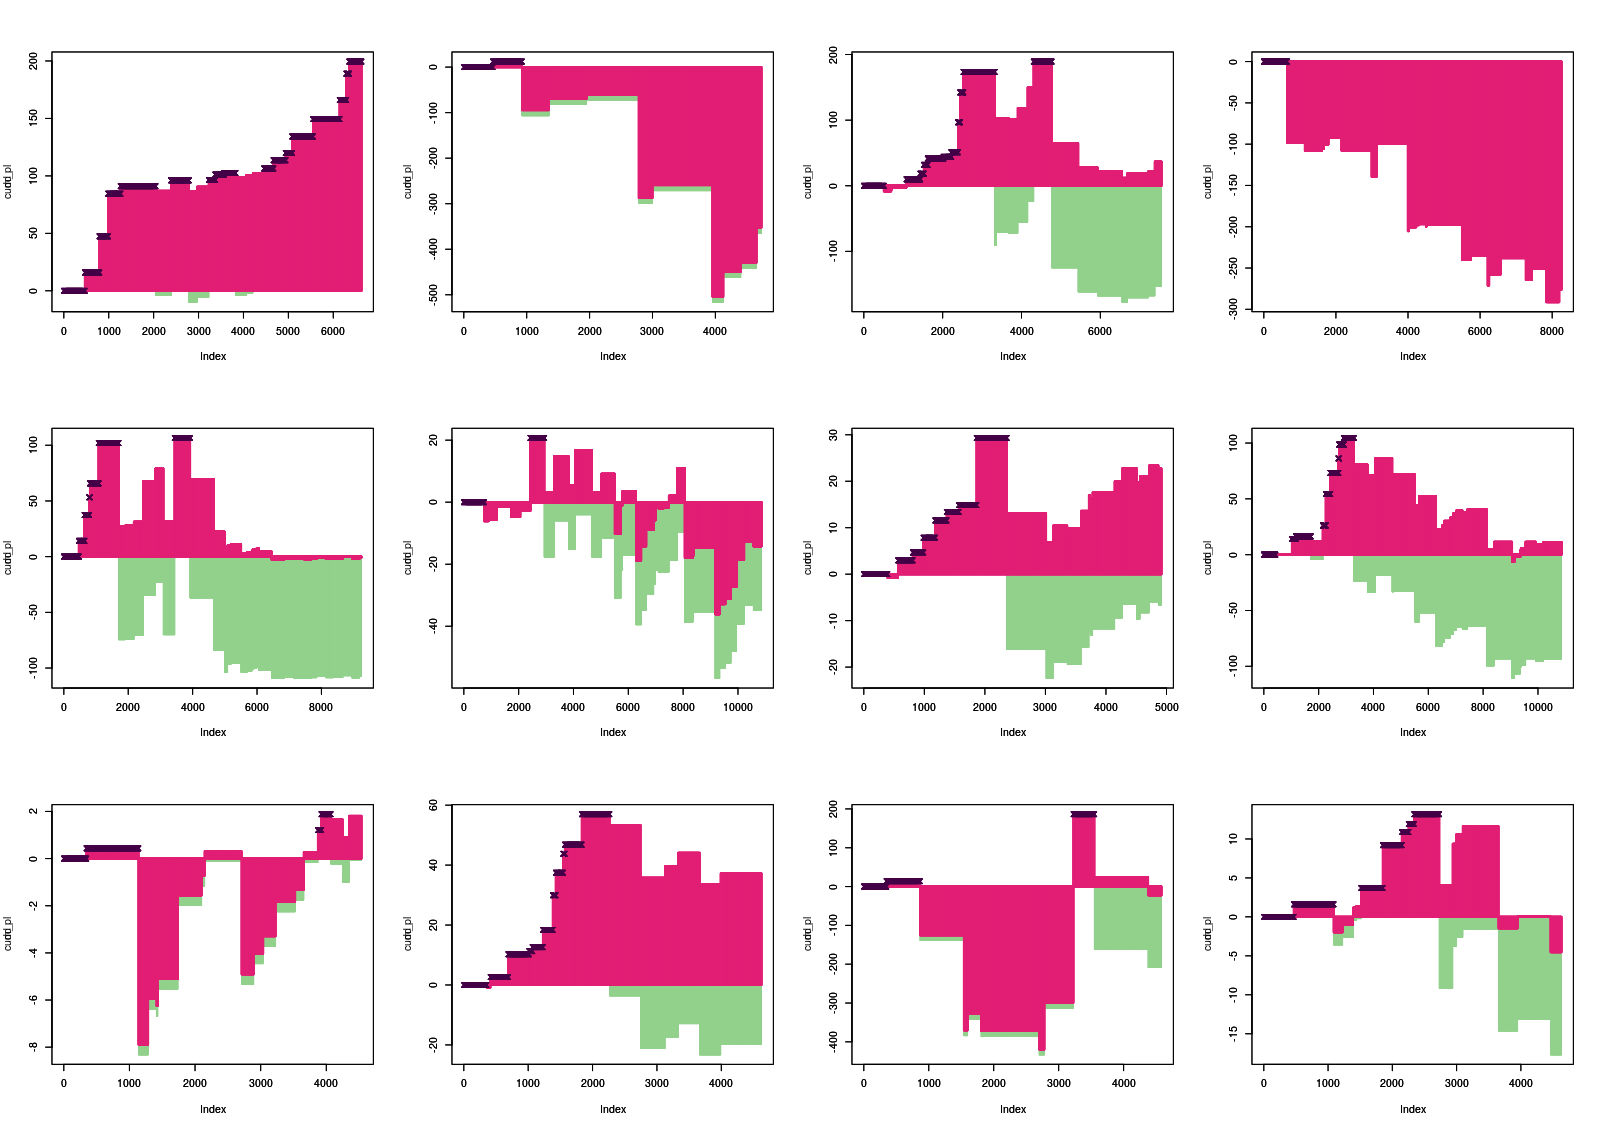
\includegraphics[width=0.75\textwidth]{sd_pl}
    \caption{Profit/loss vector of strategy D}
    \label{fig:d}
\end{figure}

\begin{table}[h!]
    \centering
    \begin{tabular}{ |c|c|c|c|c|c| }
        \hline
        Symbol & Win rate & Gain rate & Profit factor & MDD & Max DDD \\ [0.5ex]
        \hline
        2330 & 0.86 & 1.92 & 12.19 & -0.89 & 636 \\
        2454 & 0.70 & 0.16 & 0.39 & -176.52 & 1 \\
        2317 & 0.72 & 0.44 & 1.13 & -65.90 & 987 \\
        2308 & 0.56 & 0.25 & 0.32 & -162.16 & 1 \\
        2303 & 0.65 & 0.52 & 0.99 & -65.22 & 1744 \\
        1301 & 0.68 & 0.41 & 0.90 & -19.01 & 1693 \\
        2412 & 0.68 & 0.84 & 1.80 & -7.10 & 176 \\
        1303 & 0.67 & 0.51 & 1.06 & -45.41 & 603 \\
        2891 & 0.73 & 0.40 & 1.12 & -1.79 & 2734 \\
        2882 & 0.76 & 0.66 & 2.14 & -8.18 & 62 \\
        3008 & 0.40 & 1.45 & 0.96 & -192.68 & 2362 \\
        2881 & 0.76 & 0.26 & 0.85 & -3.94 & 427 \\ [0.5ex]
        \hline
    \end{tabular}
    \caption{Performance metrices of strategy D, with MDD's unit being NTD and Max DDD's unit being day}
    \label{table:d}
\end{table}

\subsection{Strategy E -- Trend trading}
Moving Average Convergence Divergence (MACD) is used in the strategy, which is calculated by subtracting the 90-day SMA of closing price of the given stock from the 65-day counterpart. The MACD's signal line is the 21-day SMA of itself. When the MACD crosses above its signal line (golden cross), we buy in at opening price on the next day, and then hold to sell out at opening price on the following day when the MACD crosses below its signal line(death cross). The performance of strategy E is demonstrated in Figure \ref{fig:e} and Table \ref{table:e}.

\begin{figure}[h]
    \centering
    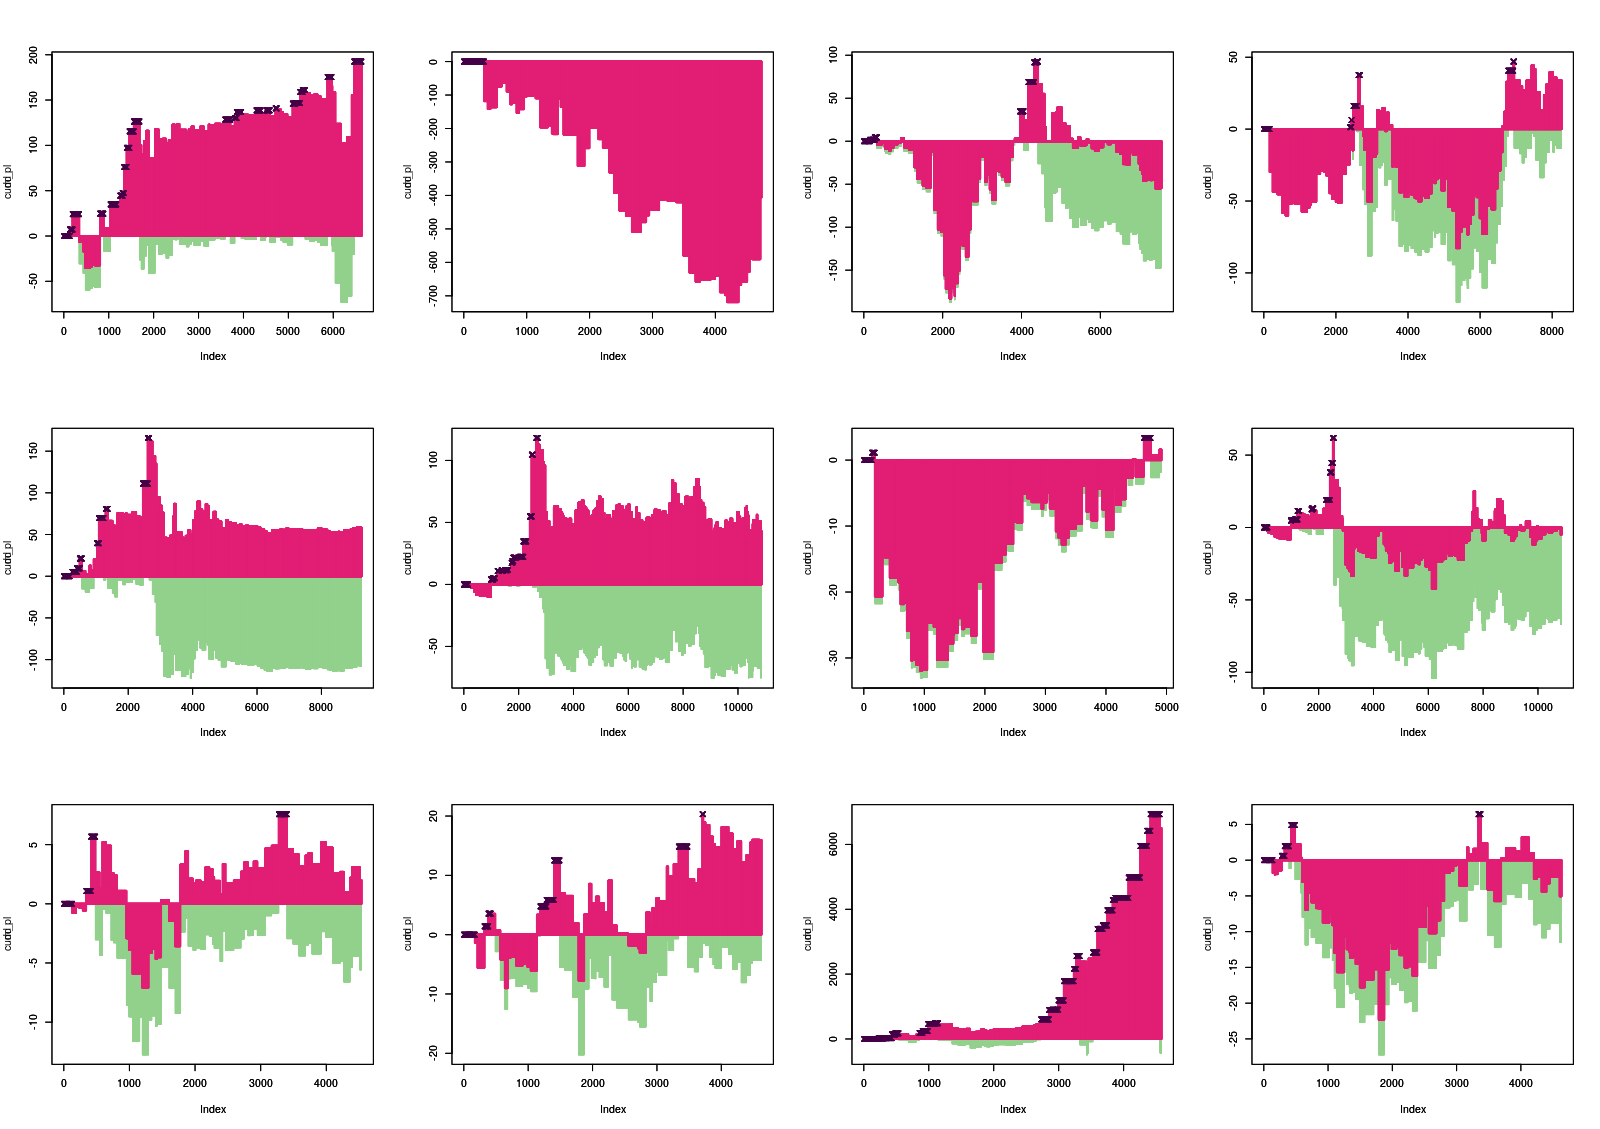
\includegraphics[width=0.75\textwidth]{se_pl}
    \caption{Profit/loss vector of strategy E}
    \label{fig:e}
\end{figure}

\begin{table}[h!]
    \centering
    \begin{tabular}{ |c|c|c|c|c|c| }
        \hline
        Symbol & Win rate & Gain rate & Profit factor & MDD & Max DDD \\ [0.5ex]
        \hline
        2330 & 0.50 & 1.60 & 1.64 & -12.95 & 1908 \\
        2454 & 0.44 & 0.83 & 0.67 & -349.40 & 1 \\
        2317 & 0.47 & 1.01 & 0.91 & -68.63 & 3629 \\
        2308 & 0.50 & 1.03 & 1.07 & -51.66 & 4115 \\
        2303 & 0.43 & 1.51 & 1.17 & -75.51 & 1095 \\
        1301 & 0.44 & 1.41 & 1.13 & -45.00 & 830 \\
        2412 & 0.49 & 1.04 & 1.01 & -15.01 & 4444 \\
        1303 & 0.47 & 1.08 & 0.98 & -56.13 & 861 \\
        2891 & 0.45 & 1.27 & 1.04 & -3.99 & 2796 \\
        2882 & 0.41 & 1.65 & 1.19 & -6.04 & 1850 \\
        3008 & 0.77 & 1.66 & 5.61 & -67.76 & 1585 \\
        2881 & 0.46 & 1.08 & 0.93 & -10.87 & 2853 \\ [0.5ex]
        \hline
    \end{tabular}
    \caption{Performance metrices of strategy E, with MDD's unit being NTD and Max DDD's unit being day}
    \label{table:e}
\end{table}

\section{Conclusion}
I have studied a lot regarding the academic field algorithmic trading through researching the paper \textit{Using Reinforcement Learning in the Algorithmic Trading Problem} and working on several strategies (to be honest, it is highly arduous tuning the parameters for these programs). I also learnt \LaTeX{} (actually, this document is written and compiled by the software system), which I found extremely helpful for my future academic career!

\medskip

\bibliographystyle{unsrt}
\bibliography{reference}

\end{document}
